%
%	background.tex
%
%	Final Report: Background
%
%	John Hughes and Michael Jean
%	University of Manitoba
%

\chapter{Background}

The vehicle as a whole is primarily a mechanical device, but carries several critical electronic control systems. Three key mechanical systems that either require electronic control or can benefit from electronic control are

\begin{itemize}
\item the \emph{internal combustion engine} (ICE\nomenclature{ICE}{Internal Combustion Engine}); 
\item the \emph{braking system}; and
\item the \emph{suspension system}.
\end{itemize}

\section{Internal Combustion Engine}
\label{sec:ice_overview}

\nomenclature{MAP}{Manifold Absolute Pressure}
\nomenclature{ECU}{Engine Control Unit}
\nomenclature{DAC}{Data Acquisition Device}
\nomenclature{GPS}{Global Positioning System}

The ICE is the stock \emph{Honda CBR600F4i} motorcycle engine. It is a 600 cm$^3$ super-sport class engine with an internal 6-speed chain driven transmission. 

\begin{figure}[H]
	\centering
	 	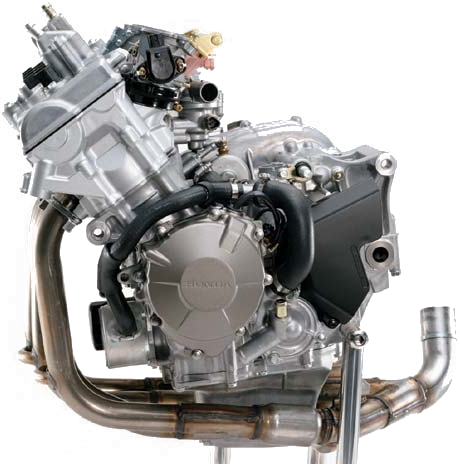
\includegraphics[scale=0.5]{Figures/cbr600f4i_engine.png}
    \caption{The Honda CBR600F4i engine.}
    \label{fig:cbr600f4i_engine}
\end{figure}

\subsection{Sensors}

The engine has a set of sensors attached to it, including

\begin{itemize}
\item an O$_{2}$ sensor;
\item a Manifold Absolute Pressure (MAP) sensor; 
\item an oil pressure sensor;
\item a water temperature sensor;
\item a throttle position sensor;
\item a gear position sensor;
\item cam and crank position sensors; and
\item an output shaft speed sensor.
\end{itemize}

\subsection{Electronic Control Possibilities}

Several tasks and responsibilities are best accomplished by electronic means, i.e.,

\begin{itemize}
\item the fuel injectors must be provided with timing signals;
\item the spark coils must be provided with firing signals;
\item a signal to engage the starter solenoid must be provided;
\item the clutch and gear selection levers must be intelligently actuated to change gears; 
\item the clutch must be intelligently actuated to enable the vehicle to move forward slowly;
\item the intake runner lengths must be modulated to provide maximum torque; and
\item sensor outputs must be logged and relayed to team members wirelessly.
\end{itemize}

\subsection{Engine Control Unit (ECU)}

A specialized third-party component called the \emph{Engine Control Unit} (ECU) controls the fuel injector and spark coil systems that in turn control the combustion cycle of the engine. The particular model of ECU used by the Formula SAE car is the S80Pro from DTAFast \cite{s80pro}. The ECU uses the O$_{2}$, MAP, cam position, and crank position sensors to adjust the fuel injector and spark coil timings. This keeps the engine running smoothly. The ECU features a traction control system that monitors wheel slip and cuts spark and fuel to provide traction when one of the wheels is slipping. The ECU also collects the various sensor readings and makes them available to other electronic devices at a fixed frequency through a shared data bus. 

\begin{figure}[H]
	\centering
	 	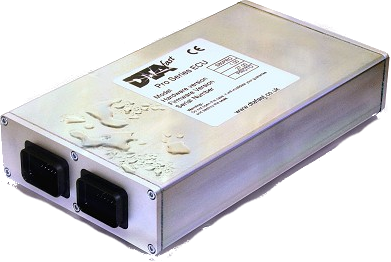
\includegraphics[scale=0.5]{Figures/s80.png}
    \caption{The DTAFast S80Pro engine control unit.}
    \label{fig:s80pro_product}
\end{figure}

\subsubsection{ECU Data interface}
\label{sec:ecu_data} 

The ECU provides 2 digital communication methods:
\begin{itemize}
 \item An RS-232 link is used by the software that DTA provides for tuning and controlling the ECU. The serial protocol that the software uses is proprietary and undocumented.
 \item A read-only CAN bus interface that emits ECU data at a fixed frequency. The message format for the CAN data is documented in Appendix \ref{cha:ecu_can_spec}.
\end{itemize}
 
\nomenclature{RS-232}{Recommended Standard 232, a byte-oriented serial communications protocol, typically asynchronous.}

\subsection{Starting the ICE}

The ICE is started by energizing a \emph{starter solenoid}. This solenoid relays a large electric current to the \emph{starter motor}, which turns over the engine and causes it to start. An external control signal from the driver must engage and disengage the starter solenoid.

\subsection{Transmission}

The ICE has an internal 6-speed manual transmission. The first, fifth, and sixth gears have been removed to reduce weight. The vehicle is not operated at speeds that would benefit from the presence of the fifth or sixth gear.

The clutch is actuated by a lever attached to the engine body. a pre-tensioned spring keeps the clutch engaged when there is no force on the lever. As force is applied to the lever, the clutch is gradually disengaged. The relationship between lever position the distance between the clutch plate and flywheel is non-linear. 

The gear selector is also actuated by a lever attached to the engine body. The gear selector may be rotated in either direction from its rest point. Up-shifting is accomplished by rotating the lever in one direction, while down-shifting is accomplished by rotating the lever in the opposite direction. 

Operating a purely mechanical manual transmission is taxing on the driver, and requires levers and linkages in the cockpit. Ideally, shifting between gears should happen as quickly as possible and require as little of the driver's attention as possible. Engagement of the clutch should be as smooth as possible.

\subsubsection{Transmission Control}
\label{sec:transmission_control_background}

Formula SAE cars designed at the University of Manitoba have utilized an electro-pneumatic shift actuation system for the past several years. This system is controlled electronically from the steering wheel by paddles. A compressed air cylinder is used to feed air to pneumatic pistons, which apply force to the levers on the clutch shaft and shift shaft. Binary solenoid valves apply pressure to either side of the pistons. 

In 2007, electronic control of the solenoid valves was realized by a set of switches on the steering wheel, which switched the low-current side of a set of relays. This in turn fed current to the solenoid valves, causing the cylinders to actuate the shift and clutch levers. In this system, the timing of the mechanical interaction with the transmission was entirely dependent on how long the driver held down the paddles. This required a lot of effort from the driver, and often resulted in missed shifts. It also caused heavy mechanical stress on the transmission. 

The 2008/2009 Formula SAE car improved on the 2007 design by replacing the relays with high-current solid state drivers. The timing signals to the solenoid valves were precisely controlled with an ARM7 micro-controller. Shift timing could be programmed, and no longer depended on how long the paddles were held. This  reduced the effort required from the driver and also reduced possible driver error.

Although an improvement from previous years, several inherent drawbacks to the 2008/2009 shift system exist. The system uses a lot of air, and the air cylinder must be regularly refilled, which is a recurring expense.

The most serious drawback of the system is that the position of the cylinders is only binary or trinary. It is only possible to engage or disengage the clutch at a constant rate, determined by the pressure in the system, the flow rate coefficient through the valves, and the diameter of the piston. To launch the car, that is, in order to smoothly increase the momentum of the car from a stand-still, requires controlling the rate at which the clutch plates return into contact with each other. This level of control is not possible with a binary pneumatic system. In order to launch the car, a hand-lever was still required.

\subsection{Intake}

The intake consists of several parts, including the \emph{throttle-body}, \emph{restrictor}, \emph{intake plenem}, \emph{intake runners}, and \emph{intake valves}. The throttle-body is a valve that controls the amount of air entering the intake system. It is followed by a restrictor, which restricts the maximum air flow into the engine. Use of a restrictor is mandated Formula SAE rules. After the restrictor, the air flows into a large intake plenum. From the plenum, four intake runners lead to each cylinder head, where the intake valves are located.

As the intake valves on the engine open, they generate negative pressure waves that travel the length of the intake runners and back into the intake plenum. There, they reflect and travel back towards the intake valve. This reflection towards the intake valves can act to increase pressure at the valve and increase power.

A fair amount of research has been done in previous years on the intake and exhaust design for the Formula SAE car. Former UMSAE engine section head Lucas Groening wrote an undergraduate thesis on modelling of the engine package for the 2008 Formula car. One important dynamic aspect of the engine design that he describes is the effect of the intake runner length on the torque output of the engine at different RPM \cite{Modelingof20}. 

From figure \ref{fig:irl_effect}, we see the two distinct torque peaks that occur at different RPMs vary depending on intake plenum length. Different plenum lengths cause the two torque peaks to occur at different RPMs. An electronic means of modulating the length of the runners to maximize engine torque would dramatically improve engine performance.

\begin{figure}[H]
	\centering
	 	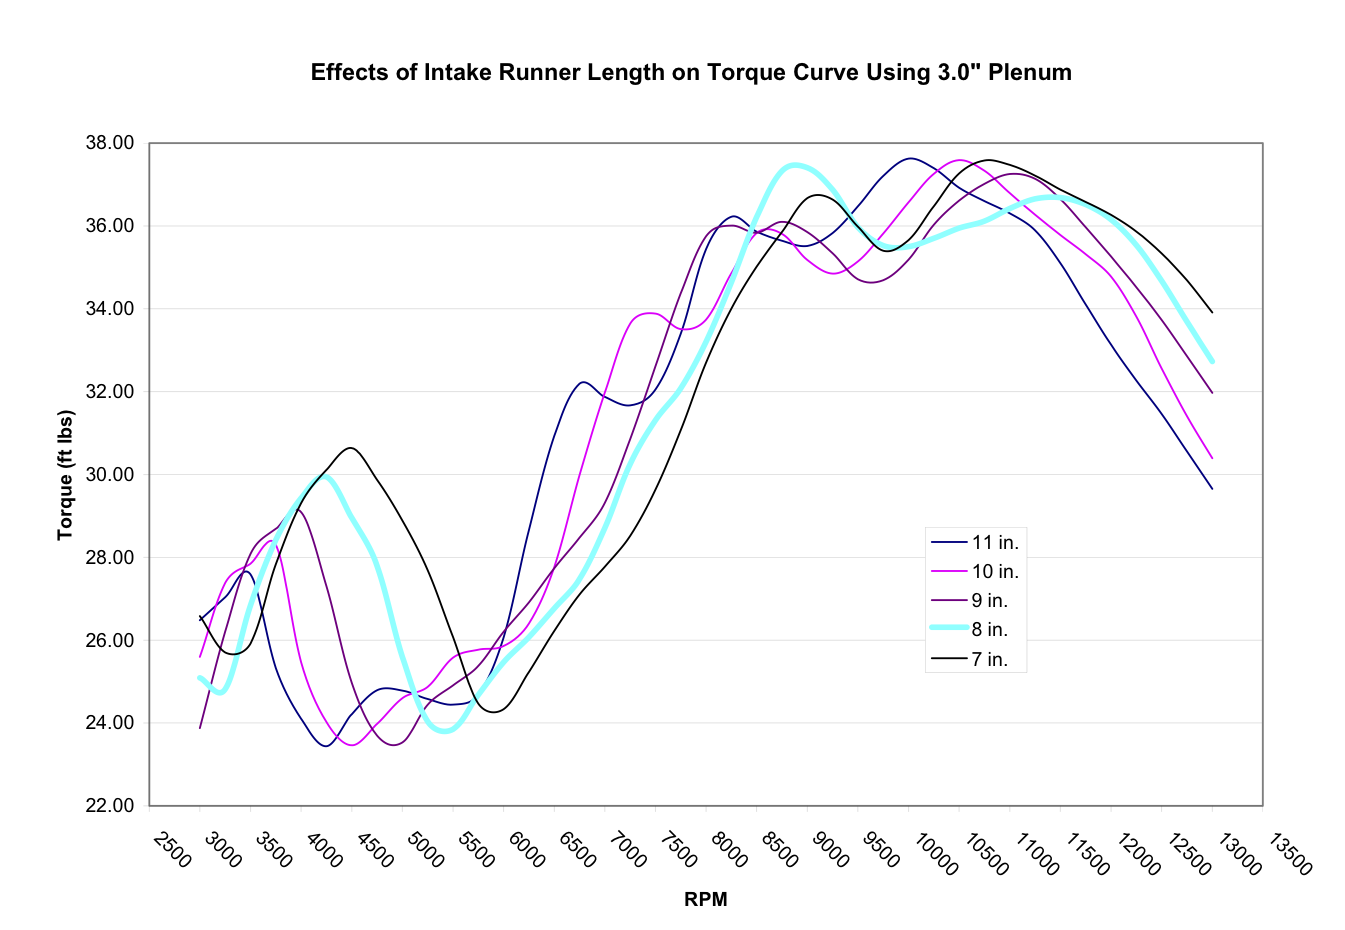
\includegraphics[scale=0.60]{Figures/irl_effect.png}
    \caption{The effect of intake runner length on torque for various RPM.}
    \label{fig:irl_effect}
\end{figure}

\subsection{Data Acquisition Device (DAC)}

Another specialized third-party component called the \emph{Data Acquisition Device} (DAC) is used to log and relay sensor data to other electronic devices.

The particular DAC used is the model DL1 from Race Technology \cite{DL1Dsheet}. The DL1 is an expandable data logger with built-in 20-Hz GPS and 3-axis accelerometer.

\subsubsection{DAC Data Interface}

Race Technology provides a software suite that communicates with the DAC using a documented serial protocol. Every item that the DAC logs is output to its own channel in real time on the serial port. It is also possible to configure the software to recognize new channels for arbitrary types of data.

\begin{figure}[H]
	\centering
	 	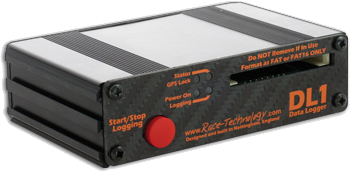
\includegraphics[scale=0.5]{Figures/dl1.png}
    \caption{The Race Systems DL1 data acquisition device.}
    \label{fig:dl1_product}
\end{figure}

\section{Braking System}
\label{sec:brake-overview}

The braking system on the 2010 Formula vehicle is a hydraulically-controlled, \emph{disc brake} system. Hydraulic pressure causes callipers on each wheel to squeeze friction pads against the discs, thus braking the vehicle. There are two entirely independent closed hydraulic systems, one for the front brakes and the other for the rear brakes. If one of the systems fails, the other system may be used to safely stop the vehicle.

\subsection{Brake Pedal, Master Cylinders and Balance Bar}

A brake pedal in the cockpit is used to engage the brakes. Two \emph{brake master cylinders} (one for the front system and the other for the rear system) are connected to the brake pedal by way of a \emph{balance bar} (see figure \ref{fig:balance_bar_diag}). The balance bar distributes force from the brake pedal to the master cylinders \cite{TiltonBrakeBias}. 

\subsection{Pressure Sensors}

Both the front and rear systems endure pressures ranging from 0 psi when the brakes are not engaged to 1000 psi when the brakes are fully engaged. Each system has it's own pressure sensor, which translates these pressures into a voltage suitable for sampling by a microcontroller.

\subsection{Brake Biasing}

Changing the relative braking force between the front and rear is called \emph{brake biasing}. For example, having 65\% of the braking force applied to the front wheels and 35\% to the rear is denoted as "65/35" brake biasing. 

Most of the vehicle weight is in the rear, where the engine is mounted. During braking, weight is effectively transferred from the rear of the vehicle to the front. This weight transfer reduces the braking force available to the rear tires. If too much rear brake force is applied, the rear tires may lock-up and the vehicle will lose traction \cite{FundVehicleDynamics}. This situation can be avoided by properly biasing the brakes for driving conditions.

\begin{figure}[h!]
	\centering
	 	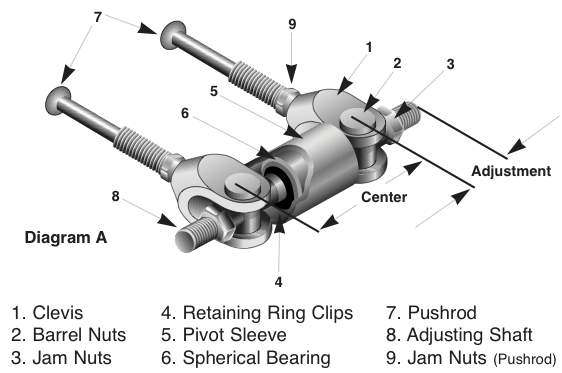
\includegraphics[scale=1.0]{Figures/balance_bar_diag.png}
    \caption{A Tilton brand balance bar, similar to that used on the Formula SAE vehicle.}
    \label{fig:balance_bar_diag}
\end{figure}

\subsection{Adjusting Shaft}

The relative force provided to each brake master cylinder can be changed by rotating an \emph{adjusting shaft} on the balance bar. When the adjusting shaft is centred between the front and rear cylinders, an equal amount of force will be applied to each. The relationship between the deviation of the adjusting shaft from it's centre position and the relative force applied to each cylinder is approximately linear for a range between 65/35 and 35/65. See table \ref{table:bb_force_distribution} for more details.

\begin{table}[H]
	\centering
	\caption{Braking force distribution.}
	\label{table:bb_force_distribution}	
	\begin{tabular}{| l | c | c |}
		\hline Adjustment Rod Position & Left Clevis & Right Clevis  \\ \hline
		\hline 3/8" left-of-centre & 65\% & 35\% \\ 
		\hline 1/4" left-of-centre & 60\% & 40\% \\
		\hline 1/8" left-of-centre & 55\% & 45\% \\
		\hline Centred & 50\% & 50\% \\
		\hline 1/8" right-of-centre & 45\% & 55\% \\
		\hline 1/4" right-of-centre & 40\% & 60\% \\
		\hline 3/8" right-of-centre & 35\% & 65\% \\
		\hline
	\end{tabular}
\end{table}

\subsection{Difficulties in Bias Adjustment}

Adjusting the brake bias in virtually all previous generations required removing body panels or the front nose cone, and manually turning a knob on the bias bar. Finding an appropriate setting for brake bias was a tedious trial and error exercise, as drivers had to run a lap in the car, brake heavily, and then return to the team so that the body could be removed and the bias adjusted. This is a very lengthy feedback loop in adjustability.

\subsection{Brake Pedal Assembly}

The brake pedal and master cylinders are attached to a \emph{brake pedal assembly} located at the end of the cockpit (see figures\ref{fig:brake_pedal_assy_a} and \ref{fig:brake_pedal_assy_b}). Removal of the brake pedal assembly is prohibited because the brake lines that connect to the master cylinder cannot be removed without depressurizing both the front and rear brake systems. 

\begin{figure}[h!]
	\centering
		\subfigure[Front view]{
			\label{fig:brake_pedal_assy_a}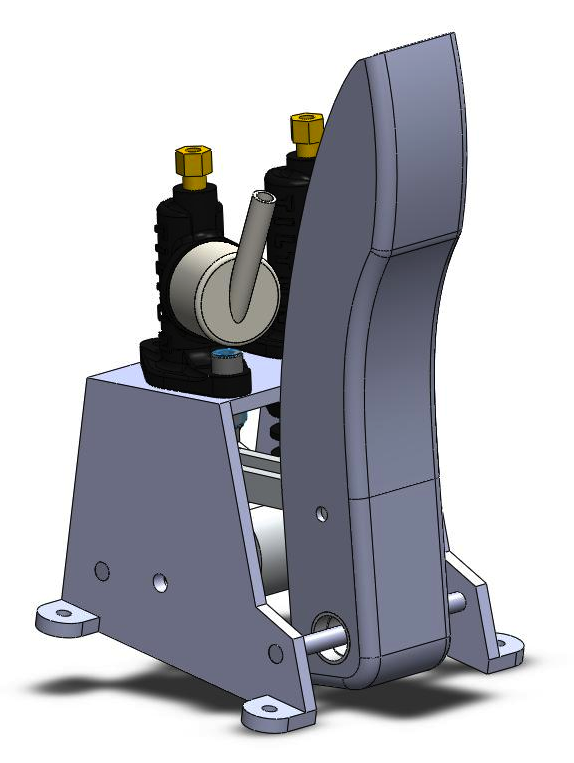
\includegraphics[scale=0.4]{Figures/brake_pedal_assy_a.png}}
		\subfigure[Rear view]{
			\label{fig:brake_pedal_assy_b}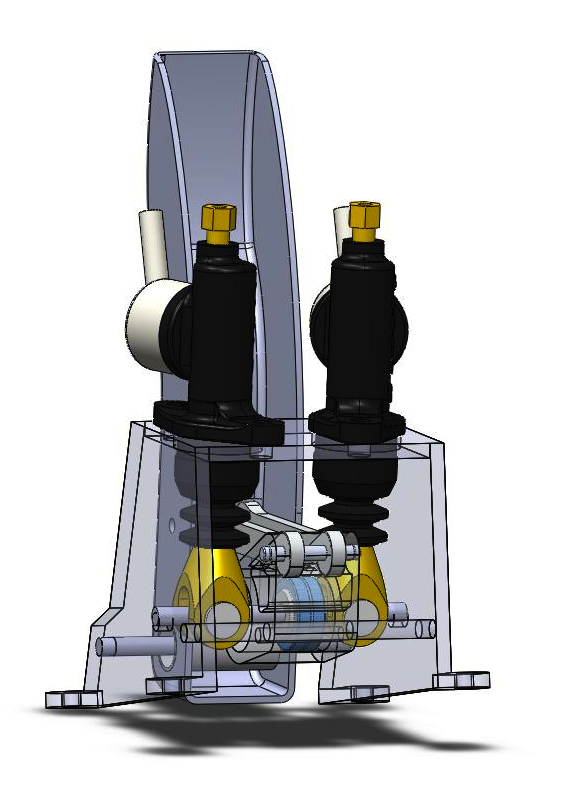
\includegraphics[scale=0.4]{Figures/brake_pedal_assy_b.png}}
    \caption{The brake pedal assembly.}
    \label{fig:brake_pedal_assy}
\end{figure}

\section{Suspension System}

The suspension system consists of springs that control the height and attack of the vehicle. Although electronic control of the suspension system is desirable, it is out of the scope of our thesis project and will be approached by future UMSAE teams.
